\chapter{Analysis with the Full Run 2 Dataset}
\label{chapter:fullRun2}

% --------------------------------------------------------------------------------------
\section{Event Selection Optimization}
- new variables (MET significance)\\
- signal/background or significance optimization, ...\\

% --------------------------------------------------------------------------------------
\section{Applying the \gjets Method to Data}

- continue efforts with the \gjets method\\
- try MET cut before reweighting?\\
- obtain weights from MC?\\
- define a validation region\\
- apply weights to data, compare with MC to test closure\\
- implementation in MonoZUVic\\

% --------------------------------------------------------------------------------------
\section{Signal Models}
- s-channel simplified models at NLO
- t-channel signals: Bell model (mediator-Z diagram), less simplified model

It should also be noted that, in the time since these initial benchmark models were set, next-to-leading order (NLO) models are now being considered instead of the leading order (LO) tree diagrams discussed here. Finally, in addition to these $s$-channel diagrams there also exist $t$-channel processes that are of great interest to the \monoZ search. These will be discussed more in Chapter \ref{chapter:fullRun2}.

% --------------------------------------------------------------------------------------
\section{Prospective Limits with 140 \ifb}

\begin{figure}[htb]
\centering
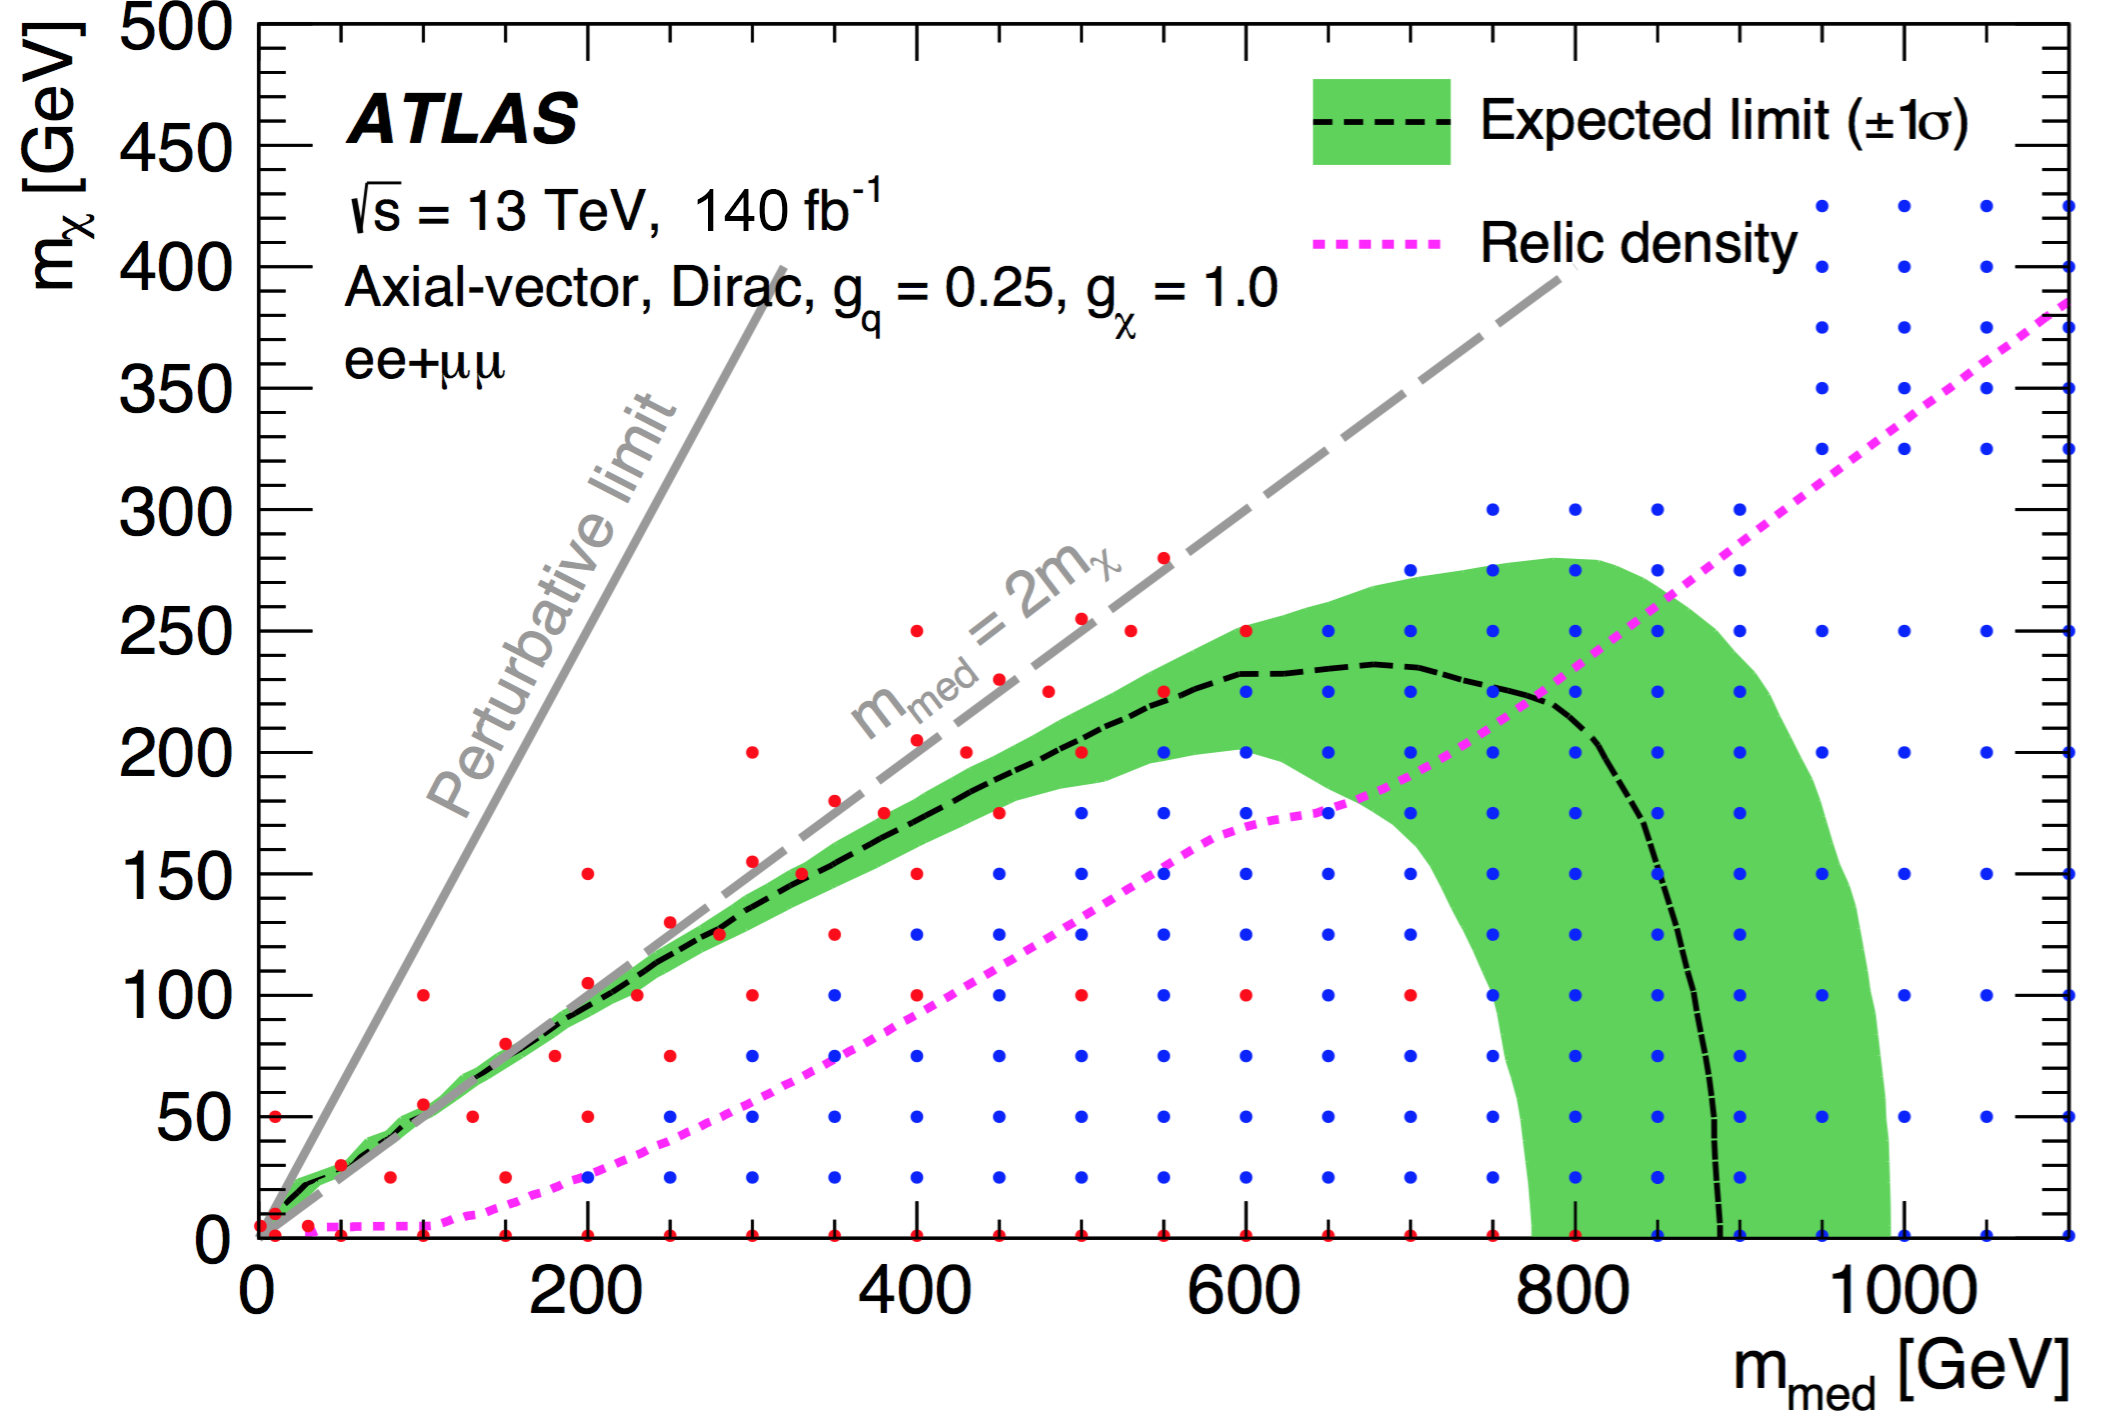
\includegraphics[width=0.7\textwidth]{Figures/140ifb.png}
\caption{Prospective vector exclusion limit with 140 \ifb. Produced by Chris Anelli.}
\label{fig:id}
\end{figure}

% --------------------------------------------------------------------------------------
\section{Other Analysis Improvements}

- comparison with ID measurements\\

\begin{figure}[htb]
\centering
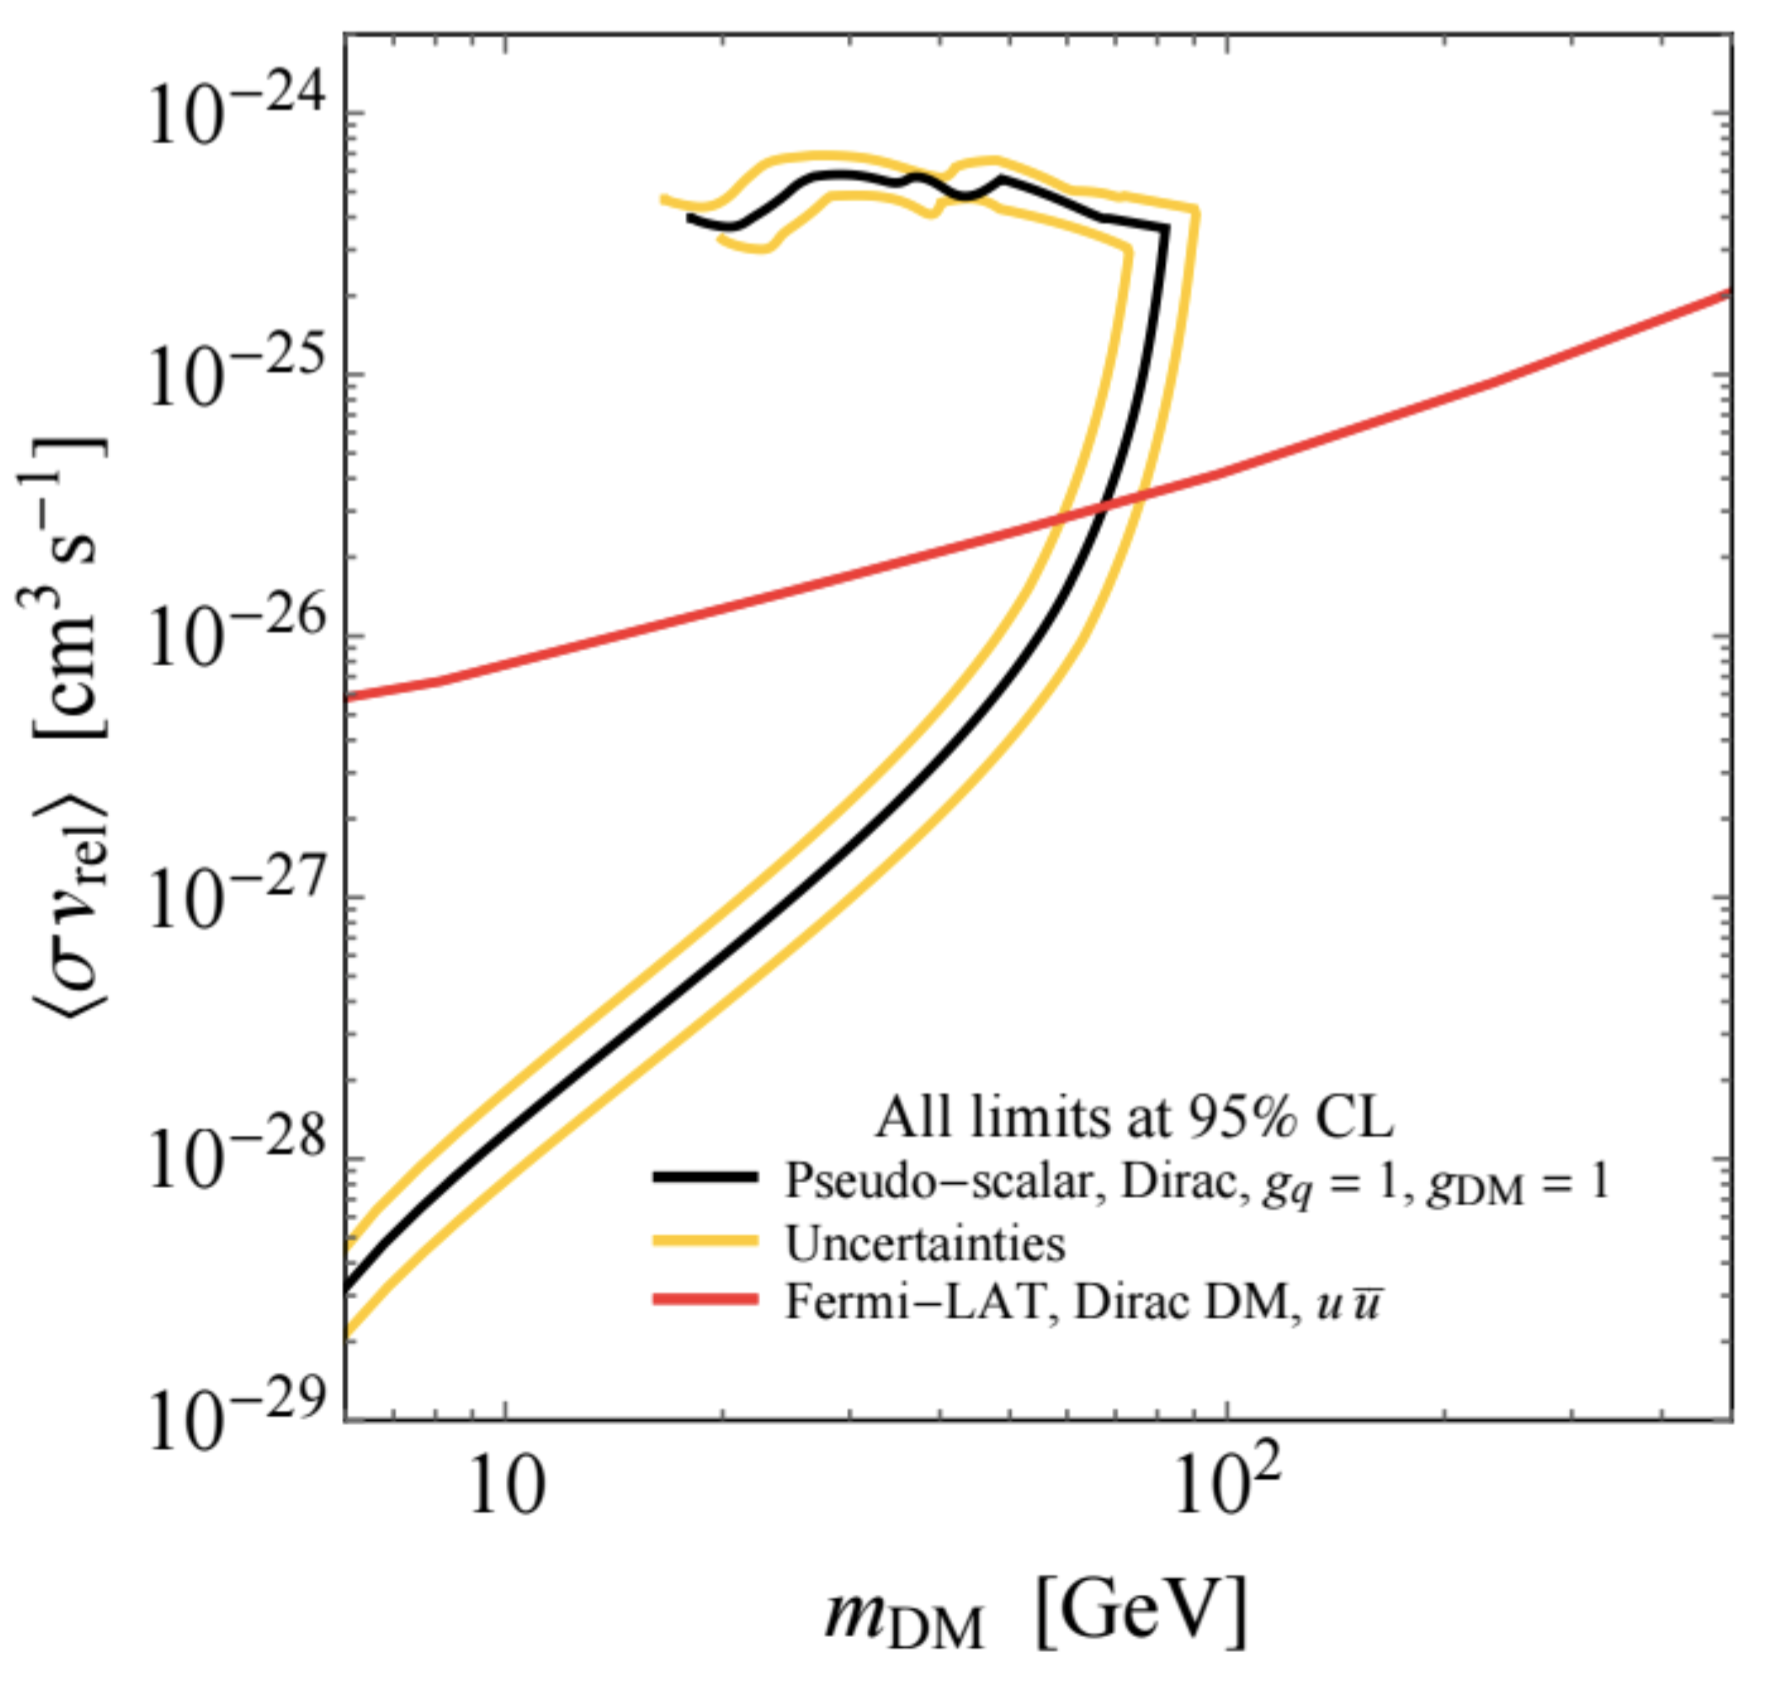
\includegraphics[width=0.5\textwidth]{Figures/id.png}
\caption{A schematic of what a comparison with ID detection measurements could look like.}
\label{fig:id}
\end{figure}

- theoretical uncertainties on signal acceptance - weights!! \\
- maintenance of analysis code\\